\documentclass[titlepage,11pt]{article}
\usepackage{comment}
\usepackage{enumitem}
\usepackage{transparent} % Untuk transparansi gambar
\usepackage{listings}
\usepackage{amsmath}
\usepackage{graphicx}
\usepackage[font=small,labelfont=bf]{caption}
\usepackage[bahasa]{babel}
\usepackage{float}
\usepackage{verbatim}
\usepackage{graphicx,tabularx,multirow}
\usepackage{xcolor}
\usepackage[onehalfspacing]{setspace}
\usepackage[
	allcolors=visigrey,
	colorlinks=true,
]{hyperref}
\usepackage[a4paper,left=2cm,right=2cm]{geometry}
% Pengaturan kutipan artikel
\usepackage[style=ieee, backend=biber]{biblatex}
%Code listing style pak akok
\definecolor{codegreen}{rgb}{0,0.6,0}
\definecolor{codegray}{rgb}{0.5,0.5,0.5}
\definecolor{codepurple}{rgb}{0.58,0,0.82}
\definecolor{backcolour}{rgb}{0.95,0.95,0.92}

\usepackage{eso-pic} % Untuk menambahkan elemen ke seluruh halaman

\newcommand\BackgroundPic{
  \put(0,0){
    \parbox[b][\paperheight]{\paperwidth}{
      \vfill
      \centering
      \transparent{0.1}
      \includegraphics[width=0.4\paperwidth,keepaspectratio]{miot.png}
      \vfill
    }
  }
}

\newcommand\BackgroundAllPages{ \AddToShipoutPicture*{\BackgroundPic} }
\newcommand\BackgroundNone{ \ClearShipoutPicture } % hilangkan background

\lstdefinestyle{mystyle}{
	backgroundcolor=\color{backcolour}, commentstyle=\color{codegreen},
	keywordstyle=\color{magenta},
	numberstyle=\small\color{codegray},
	stringstyle=\color{codepurple},
	basicstyle=\ttfamily\footnotesize,
	breakatwhitespace=false,         
	breaklines=true,                 
	captionpos=t,                    
	keepspaces=true,                 
	numbers=left,                    
	numbersep=5pt,                  
	showspaces=false,                
	showstringspaces=false,
	showtabs=false,           
	frame = single,
	tabsize=2
}
\lstset{style=mystyle}

\definecolor{visigrey}{rgb}{.1,.15,.15}
\geometry{top=1cm,bottom=.5cm}
\savegeometry{titlepage}
\geometry{top=2cm,bottom=2cm}
\savegeometry{main}

\def\bspace{\(\qquad\qquad\qquad\)}
\usepackage[T1]{fontenc}
\usepackage[utf8]{inputenc}
\usepackage{tgheros}
\renewcommand*\familydefault{\sfdefault}

\setcounter{tocdepth}{6}

\def\autor{Laboratorium }
\def\lab{Multimedia dan Internet of Things}
\def\departemen{Departemen Teknik Komputer}
\def\institut{Institut Teknologi Sepuluh Nopember}
\def\praktikum{Laporan Sementara \\ Praktikum Jaringan Komputer}
\def\nama{Atria Caesariano Tinto - 5024231068}
% Ubah Judul sesuai dengan modul
\def\judul{Crimping dan Routing IPv4}
\def\tanggal{2025}
\begin{document}
% Ubah Bahasa sesuai dengan keinginan
\selectlanguage{bahasa}

\BackgroundNone
\def\headingtype{\bf \small}
\loadgeometry{titlepage}

\begin{titlepage}
	\centering
	\begin{tabularx}{\textwidth}{l@{\hskip 0pt}lX}
		\raisebox{-0.5\height}{
\includegraphics[width=3cm]{Cover/img/logodepart.png}} 
		& \raisebox{-0.5\height}{\includegraphics[width=3cm]{Cover/img/miot.png}} 
		& \raggedleft
	\hfill
	\begin{minipage}{0.5\textwidth}
		\raggedleft
		{\emph{\headingtype \autor}} \\[-2pt]
		{\headingtype \lab} \\[-2pt]
		{\headingtype \departemen} \\[-2pt]
		{\headingtype \emph{\institut}}
	\end{minipage}

	\vspace{5cm}
	\end{tabularx}
	
	\vspace{5cm}
	{\Huge \bf \praktikum \par}
	
	\vspace{2cm}
	{\LARGE \bf \judul \par}
	
	\vspace{2cm}
	{\Large \nama \par}
	
	\vfill
	{\Large \tanggal \par}
	
	\vfill
	
\includegraphics[width=\textwidth]{Cover/img/footer.png}
\end{titlepage}

\loadgeometry{main}


\BackgroundAllPages
% Pilih Modul yang akan di build
\section{Pendahuluan}
\subsection{Latar Belakang}
Jaringan komputer merupakan aspek fundamental dalam dunia teknologi informasi yang semakin berkembang, di mana pemahaman tentang jaringan menjadi sangat penting untuk memenuhi kebutuhan komunikasi yang cepat dan efisien. Praktikum ini dilaksanakan untuk memberikan pemahaman mendalam mengenai konsep dasar jaringan komputer, termasuk jenis-jenis jaringan, protokol komunikasi, serta cara menghubungkan perangkat melalui kabel dan router. Dalam era digital, hampir semua aktivitas manusia, baik dalam bisnis, pendidikan, maupun kehidupan sehari-hari, bergantung pada jaringan komputer, sehingga pemahaman yang baik tentang jaringan sangat penting untuk memfasilitasi komunikasi yang efektif dan pengelolaan data yang efisien. Selain itu, dengan memahami jaringan, individu dapat lebih baik dalam mengelola dan mengamankan data yang dikirimkan, melindungi informasi sensitif dari ancaman cyber. Keterkaitan dengan aplikasi dunia nyata sangat jelas, di mana perusahaan mengandalkan jaringan untuk menghubungkan berbagai departemen dan lokasi, meningkatkan produktivitas dan efisiensi operasional. Di lingkungan pendidikan, jaringan komputer memungkinkan akses ke sumber daya belajar secara online dan kolaborasi antar siswa. Dengan kemajuan teknologi seperti Internet of Things (IoT), pemahaman tentang jaringan komputer menjadi semakin relevan, karena banyak perangkat pintar yang terhubung melalui jaringan. Melalui praktikum ini, diharapkan peserta dapat memahami dan mengaplikasikan konsep-konsep dasar jaringan komputer serta mampu mengatasi permasalahan yang mungkin timbul dalam pengelolaan jaringan di dunia nyata.

\subsection{Dasar Teori}
Praktikum jaringan komputer didasarkan pada beberapa teori dan konsep teknis yang mendasari cara kerja jaringan serta interaksi antar perangkat. Salah satu konsep dasar adalah jaringan komputer itu sendiri, yang merupakan kumpulan perangkat yang terhubung untuk berbagi informasi dan sumber daya. Jaringan ini dapat dibedakan menjadi beberapa jenis, seperti Personal Area Network (PAN), Local Area Network (LAN), Campus Area Network (CAN), Metropolitan Area Network (MAN), dan Wide Area Network (WAN), yang masing-masing memiliki karakteristik dan jangkauan yang berbeda.

Dalam jaringan komputer, protokol komunikasi berfungsi sebagai aturan yang mengatur bagaimana data dikirim dan diterima antar perangkat. Beberapa protokol penting yang akan dipelajari dalam praktikum ini meliputi Transmission Control Protocol (TCP), yang memastikan data dikirim dengan urutan yang benar dan tanpa kerusakan, serta Internet Protocol (IP), yang memberikan alamat unik untuk setiap perangkat dalam jaringan. Alamat IP ini terbagi menjadi dua jenis, yaitu Private IP Address dan Public IP Address, yang masing-masing memiliki fungsi dan penggunaan yang berbeda dalam konteks jaringan.

Selain itu, pemahaman tentang subnetting dan subnet mask juga sangat penting. Subnetting adalah proses membagi jaringan besar menjadi beberapa jaringan kecil untuk meningkatkan efisiensi dan keamanan. Subnet mask digunakan untuk menentukan bagian mana dari alamat IP yang menunjukkan jaringan dan bagian mana yang menunjukkan perangkat di dalam jaringan. Konsep prefix juga terkait erat dengan subnetting, di mana prefix menunjukkan berapa banyak bit dari alamat IP yang digunakan untuk Network ID.

%===========================================================%
\section{Tugas Pendahuluan}

\begin{enumerate}
	\item \textbf{Alokasi IP Address dan Prefix (CIDR)}
	
	Menggunakan jaringan privat: 192.168.0.0/24

	\textbf{> Departemen R\text{\&}D}

Jumlah perangkat: 100

Prefix CIDR: /25

Alamat network: 192.168.0.0

Rentang IP: 192.168.0.1 – 192.168.0.126

Broadcast: 192.168.0.127

\textbf{> Departemen Produksi}

Jumlah perangkat: 50

Prefix CIDR: /26

Alamat network: 192.168.0.128

Rentang IP: 192.168.0.129 – 192.168.0.190

Broadcast: 192.168.0.191

\textbf{> Departemen Administrasi}

Jumlah perangkat: 20

Prefix CIDR: /27

Alamat network: 192.168.0.192

Rentang IP: 192.168.0.193 – 192.168.0.222

Broadcast: 192.168.0.223

\textbf{> Departemen Keuangan}

Jumlah perangkat: 10

Prefix CIDR: /28

Alamat network: 192.168.0.224

Rentang IP: 192.168.0.225 – 192.168.0.238

Broadcast: 192.168.0.239

Total subnet yang diperlukan adalah 4 subnet, masing-masing untuk satu departemen.

\item jawaban

	\item Tabel Routing Sederhana
		\begin{table}[ht]
		\centering
		\begin{tabular}{|c|c|c|c|c|}
		\hline
		Network Destination & Netmask/Prefix 2 & Gateway & Interface Tujuan \\ \hline
		192.168.0.0 & 255.255.255.128 (/25) & 192.168.1.1 & eth0 (R\text{\&}D) \\ \hline
		192.168.0.128 & 255.255.255.192 (/26) & 192.168.1.1 & eth1 (Produksi) \\ \hline
		192.168.0.192 & 255.255.255.224 (/27) & 192.168.1.1 & eth2 (Administrasi)  \\ \hline
		192.168.0.224 & 255.255.255.240 (/28) & 192.168.1.1 & eth3 (Keuangan)  \\ \hline
		\end{tabular}
		\caption{Tabel routing sederhana}
		\end{table}
	
	\item Jenis Routing yang paling cocok adalah Static Routing, karena:
	
	- Jaringan kecil (hanya 4 subnet).
	
	- Perubahan topologi jarang terjadi.
	
	- Konfigurasi sederhana dan efisien.
	
	- Tidak memerlukan protokol dinamis atau overhead tambahan.
	
	Dalam skalabilitas Dynamic Routing dapat dipertimbangkan dengan protokol seperti RIP v2 atau lebih baik OSPF, karena:
	
	- CIDR-aware (tidak membatasi classful).
	
	- OSPF mendukung skala besar dan konvergensi cepat.
\end{enumerate}

\end{document}